\documentclass{genai}
\usepackage{xspace}

\title{Stable Diffusion 3 Paper Writeup}
\author{Due: Wednesday, March 13}
\date{Jack Bosco}

\begin{document}

\newcommand{\modelname}{\textbf{MM-DiT}\xspace}

\head{CSCI-297 Generative AI}{Cody Watson}

\renewcommand{\labelenumii}{\arabic{enumi}.\arabic{enumii}}
\renewcommand{\labelenumiii}
{\arabic{enumi}.\arabic{enumii}.\arabic{enumiii}}
\pagestyle{fancy}
\newpage

\maketitle

\subtitle

\begin{center}
	\begin{figure}[h]
		\centering
		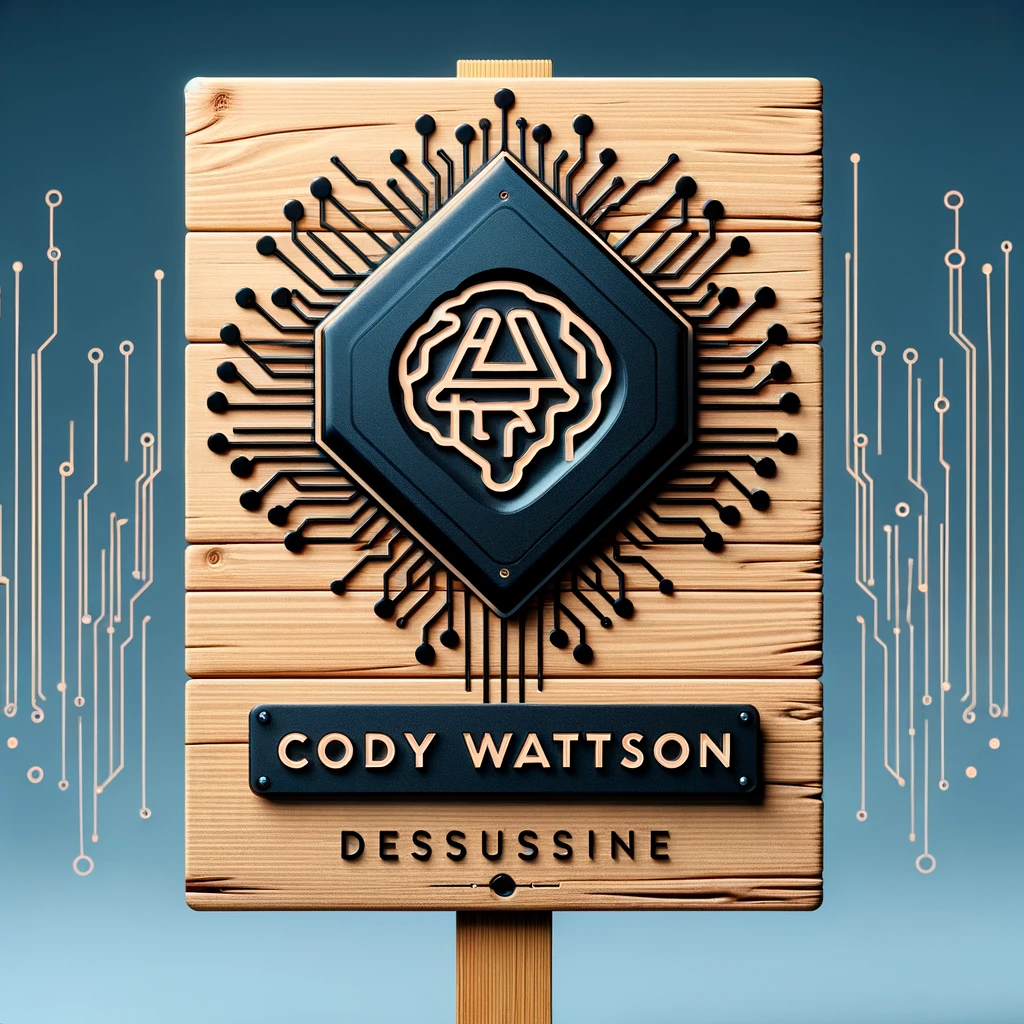
\includegraphics[width=1\textwidth]{class_logo.png}\\
		\small Image Credit: ChatGPT
	\end{figure}
\end{center}

\newpage

\section{Problem}

\hspace{\parindent} The standard way to train text-to-image (TTI) models is to fine tune gradients for an ODE (ordinary differential function). This function is differential because it must define a set of mappings tranforming text embeddings into image embeddings. The issue with this method is the curvature of common ODEs. More complex curvatures necessitate more steps to calculate the error; as a result, the model trains slower. From a broad scope, this issue makes training TTI models at scale expensive both in terms of time and money.

A recent breakthrough in generative modeling called Rectified Flow (RF) constructs a mapping between image and text gradients with a probability distribution. In RF the data distribution is mapped to a normal distribution using straight paths, and the slopes of these paths with respect to time defines the parameters of the model. Since the paths are straight, it takes less steps to get the gradient of RF than with a derivative of a traditional ODE. Thus RF models are cheaper to train.

While this breakthrough is exciting, RF hasn’t caught steam due to its limited ability to contextual input text. With current implementations of RF, the prompt or text input is reduced to a set of classes and sequenced with a timestep: losing much of the context in the process. 

To promote the wider adoption of Rectified Flow in TTI models, the efficiency of Rectified Flow needs to be shown in a large-scale study. Training text-to-image models with RF at scale is difficult. As the image resolution increases so does the complexity of the image embeddings, implying the complexity of the text embeddings has to scale with it. With inadequate image embeddings, attention entropy declines leading to overfitting and the model’s loss falls into a local minimum. Therefore the contextualization limits of RF models limits their ability to be trained at scale.

\section{Solution}

\hspace{\parindent} In order to perform a large-scale study on RF, something has to change in the architecture to improve scalability.
The authors propose \modelname architectures, building off of previously proposed DiT architectures, as a means of allowing bidirectional Rectified Flow of the gradient.
When proposing \modelname s, the authors point out a fundamental flaw in the architecture of traditional DiTs which take in a current timestep t and a class embedding of the text $c_\text{vec}$; that is, traditional DiTs can only learn from a coarse-grained representation of the input.
Before it is fed into the DiT module, $c_\text{vec}$ is element-wise added to a MLP-representation of a sinusoidal encoding of the timestamp t allowing $c_\text{vec}$ to serve as the timestep for the DiT module.


With \modelname s, an additional contextual embedding $c_\text{ctxt}$ is introduced as an input to the architecture. Unlike $c_\text{vec}$, $c_\text{ctxt}$ provides sequential context with an additional representation from the T5-v1.1-XXL frozen pre-trained text model. This allows for more fine-grained contextualization of the prompt: an optimization on the overall model. 

A 2x2-pixel region of noise’s latent space x is the third and final input to the \modelname . The inclusion of an encoding of image data is what makes the data distributions of \modelname s multimodal and is the primary optimization on traditional DiTs. It also raises more issues since the encodings of sequential data (text) and spatial data (images) are widely different. 

The authors address this with a dual-transformer architecture: one transformer for text and one for image encodings. As inputs cctex and x progress through the architecture they are fed through separate but mirrored hidden layers. Specifically, they are fed through a normalization layer, combined with the timestep and finally fed through a linear transformation layer before being concatenated and fed to the attention module. This is how bi-directional flow differs from U-net architectures: both K and Q inputs to the attention mechanism contain both text and image data.

Since the model needs to learn different representations for the image and text data, separating the channels for image and text data is imperative for generating coherent images. Bidirectional flow is achieved in the attention layer, allowing for the model to learn both text and image representations. Learning both, \modelname s overcome the aforementioned limitation of RF – where they can’t understand complex text prompts – while preserving the optimization in training cost.

Lastly, the normalization of latent image and text representations makes scaling the model more feasible. This small optimization inside the \modelname  architecture allows for more high-definition images to be produced with less artifacting while also reducing the ability for the model to overfit to the training data.


\section{Results}

\hspace{\parindent}This paper presents a large-scale experiment for multiple models, including rectified flow and others, to test which could produce the best results.
Tests were controlled for the optimization algorithm, the model architecture, the dataset and samplers.
Models were assessed using \texttt{CLIP} and \texttt{FID} scores.
Higher scores are good on the \texttt{CLIP} scale whereas lower scores are good on the \texttt{FID} scale. 
Rectified Flow models using lognorm flow trajectory performed the best in general. 
Non-RF models such as edm and eps/linear underperformed. 
Moreover, the \texttt{rf/lognorm(0.00, 1.00)} model was able to consistently hold onto an average validation score ranking of less than 1.6 after only 5 training steps,
meaning the \texttt{rf/lognorm(0.00, 1.00)} trains faster than any other model in the study.

\begin{figure}[h]
	\centering
	
\includegraphics[height=3in]{sd3_examples.png}
\end{figure}

Most interestingly, the new bi-directional flow models are very good at generating images with text.
The above samples are a blatant reference to the book “Hitchikers Guide to the Galaxy''.
As you can see, text gets better as the images move down vertically.
This is to demonstrate the effectiveness of DPO finetuning: another name for using human feedback to finetune the model formerly known as Reinforcement Learning from Human Feedback (RLHF).
The only way to get the data necessary for RLHF is by convincing (or tricking) people into evaluating the model and using that loss for fine tuning in a RL setting. 

Speaking of “Hitchikers Guide to the Galaxy'', I thought about training my own Marv the depressed LLM someday.
The way I'd approach leveraging RLHF for finetuning Marv would be deploying him to a web forum and have him respond to people.
The environment is the chat thread, the action is Marv’s response, and reward is approximated with sentiment analysis of the replies to his response.

Anyways, the text in the images above is clearly readable.
This is a huge improvement on previous diffusion models which are hardly able to spell.
Overall the bi-directional rectified flow optimization offers huge benefits to scalability, cheapness of training and overall quality of the model.
In the \LaTeX \space source, the authors used \textbackslash\texttt{modelname} as a macro for \modelname inferring that is what they intend to name their optimized diffusion model.
However, I believe the model's outstanding results motivate a more general term for it: Stable Diffusion 3.


\end{document} 
